\documentclass[border=2pt]{standalone}
\usepackage{tikz}
\usepackage{pgfplots}\pgfplotsset{compat=1.18}
\usetikzlibrary{arrows.meta,positioning,backgrounds,fit,shapes.geometric,calc}
\definecolor{wacvblue}{rgb}{0.21,0.49,0.74}
\newcommand{\vs}{vs.\ }
\begin{document}
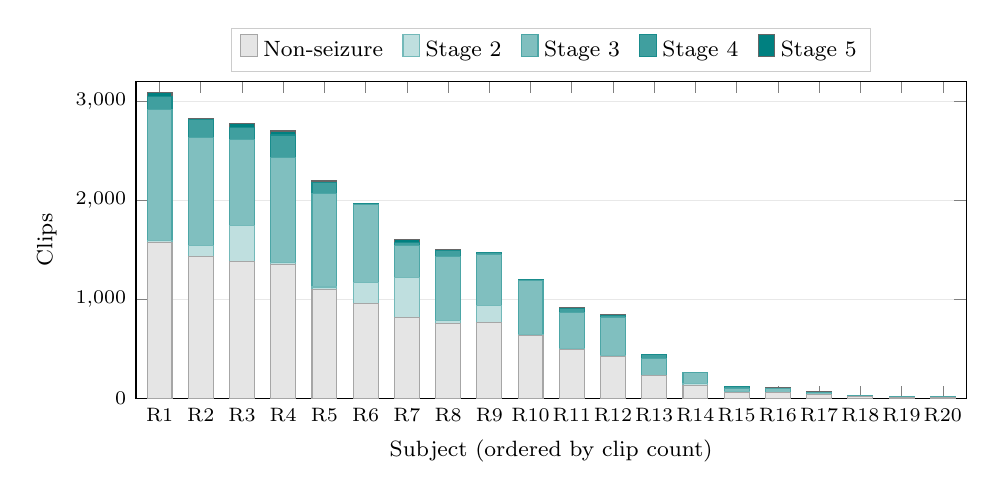
\begin{tikzpicture}
\begin{axis}[
  width=\textwidth, height=5.6cm,
  ybar stacked, bar width=9pt,
  symbolic x coords={R1,R2,R3,R4,R5,R6,R7,R8,R9,R10,R11,R12,R13,R14,R15,R16,R17,R18,R19,R20},
  xtick=data,
  x tick label style={font=\scriptsize},
  ymin=0, ymax=3200,
  ylabel={Clips},
  xlabel={Subject (ordered by clip count)},
  tick label style={font=\scriptsize},
  label style={font=\footnotesize},
  ymajorgrids, grid style={gray!18, line width=0.3pt},
  legend style={font=\footnotesize, at={(0.5,1.03)}, anchor=south,
                legend columns=-1, draw=gray!40,
                /tikz/every even column/.append style={column sep=5pt}},
  enlarge x limits=0.03,
]
\addplot[fill=black!10, draw=black!35] coordinates {(R1,1576)(R2,1431)(R3,1380)(R4,1351)(R5,1100)(R6,955)(R7,814)(R8,754)(R9,763)(R10,631)(R11,491)(R12,422)(R13,224)(R14,131)(R15,59)(R16,53)(R17,32)(R18,17)(R19,7)(R20,6)};
\addplot[fill=teal!25, draw=teal!55] coordinates {(R1,22)(R2,113)(R3,364)(R4,22)(R5,23)(R6,218)(R7,408)(R8,33)(R9,177)(R10,16)(R11,6)(R12,10)(R13,2)(R14,12)(R15,3)(R16,4)(R17,1)(R18,0)(R19,0)(R20,1)};
\addplot[fill=teal!50, draw=teal!70] coordinates {(R1,1325)(R2,1094)(R3,873)(R4,1062)(R5,946)(R6,782)(R7,317)(R8,648)(R9,511)(R10,544)(R11,364)(R12,387)(R13,174)(R14,112)(R15,39)(R16,36)(R17,25)(R18,9)(R19,4)(R20,4)};
\addplot[fill=teal!75, draw=teal!90] coordinates {(R1,131)(R2,181)(R3,124)(R4,226)(R5,114)(R6,8)(R7,36)(R8,61)(R9,21)(R10,6)(R11,47)(R12,20)(R13,42)(R14,3)(R15,16)(R16,7)(R17,2)(R18,2)(R19,3)(R20,0)};
\addplot[fill=teal!100!black, draw=black!60] coordinates {(R1,37)(R2,11)(R3,33)(R4,40)(R5,12)(R6,0)(R7,25)(R8,6)(R9,2)(R10,2)(R11,10)(R12,2)(R13,2)(R14,4)(R15,1)(R16,3)(R17,2)(R18,1)(R19,0)(R20,0)};
\legend{Non-seizure, Stage 2, Stage 3, Stage 4, Stage 5}
\end{axis}
\end{tikzpicture}
\end{document}
